\documentclass[a4paper,12pt]{report}

\usepackage[lmargin=2.00000cm,rmargin=2.0000cm,tmargin=5.5000cm,bmargin=2.500000cm,headheight=3.5cm]{geometry}        %Flexible and complete interface to document dimensions
\usepackage[utf8]{inputenc}
\usepackage[T1]{fontenc}
%\usepackage[latin1]{inputenc}
\usepackage{amsmath}
\usepackage{amsfonts}
\usepackage{amssymb}
\usepackage{lmodern}
\usepackage{float}
\usepackage{graphicx}

\usepackage[english,french]{babel}        %use for the below package `datetime'
\usepackage[babel=true]{csquotes}
\usepackage{datetime}        %Change format of `\today' with commands for current time
\renewcommand{\dateseparator}{-}
\newcommand{\headertoday}{\twodigit\day \dateseparator \twodigit\month  \dateseparator \the\year}

\usepackage{animate}
\usepackage{lastpage}
\usepackage{array}
\usepackage{lastpage}
\usepackage{multirow}
\usepackage{titling}
\usepackage{placeins}
\usepackage{media9}
\usepackage{eurosym}
\usepackage{pdflscape}
\usepackage{color}
\usepackage[table]{xcolor}
\definecolor{mon_bleu}{rgb}{0.137,0.466,0.741}
\definecolor{mon_vert}{rgb}{0.07843,0.4627,0.07843}
\definecolor{mon_rouge}{rgb}{0.62745,0.16078,0.27058}		
%\usepackage{subfigure}
\usepackage{subcaption}

\usepackage[ 
           hidelinks,
           colorlinks=true,
           linkcolor=blue,          % color of internal links (change box color with linkbordercolor)
    	   citecolor=blue,        % color of links to bibliography
    	   filecolor=blue,      % color of file links
    	   urlcolor=blue,           % color of external links
           pdfhighlight =/O]{hyperref}																		% dvipdfm package pour lien hypertextes dans pdf (pdfhighlight--> afficher la main dans le pdf, colorlinks--> colorlinks=true afficher les liens en couleurs)
  
\usepackage{blindtext}
\usepackage[final]{pdfpages}
\usepackage[french]{cleveref}																				% à placer après hyperref attention ne pas utiliser ":" dans les labels des équations avec French babel activé et cref

\usepackage{fancyhdr}
%%%%%%%%%%%%%%%%%%%%%%%%%%%%%%%%%%%%%%%%%%%%%%%%%%%%%%%%%%%%%%%%%%%%%%%%%%
%                         FORMAT PERSONNALISES                           %
% %%%%%%%%%%%%%%%%%%%%%%%%%%%%%%%%%%%%%%%%%%%%%%%%%%%%%%%%%%%%%%%%%%%%%%%%

\parindent=0pt        %leading space for paragraphs
\pagestyle{fancy}
\renewcommand{\arraystretch}{1.5}
\renewcommand{\headrulewidth}{0pt}
\fancyhead[CE,CO,LE,LO,RE,RO]{} %% clear out all headers
\fancyhead[C]{%
\begin{tabular}{|m{3.0cm}|m{10cm}|c@{}|}
\hline
\multirow{2}{*}{\includegraphics[scale=0.045]																			% LOGO LABO
{Logo-Symme.png}}& \centering \multirow{2}{*}{ \Large{\thetitle}}  &  \multirow{2}{*}{Page: \thepage ~/ \pageref{LastPage}}\\
& &  \\
\hline
%Etabli par: \newline \theauthor & \multicolumn{2}{l|}{Diffusion: interne}\\
%\hline
\multicolumn{2}{|l|}{Objet: \thetitleobject }& Date: \headertoday ~~\\ 
\hline
\end{tabular}
}
\renewcommand\footrulewidth{1pt}
\fancyfoot[L]{Document confidentiel} 																		% DOCUMENT CONFIDENTIEL
\fancyfoot[R]{Laboratoire SYMME}		 																	% NOM DU LABO

\newcolumntype{x}[1]{>{\centering\hspace{0pt}}p{#1}}
\setlength{\doublerulesep}{\arrayrulewidth} 


\usepackage{tikz}																							% pour les diagrammes
\usetikzlibrary{calc}
\usetikzlibrary{shapes.geometric,shapes.arrows,decorations.pathmorphing}
\usetikzlibrary{matrix,chains,scopes,positioning,shapes,arrows,fit}
\usetikzlibrary{calc,decorations.pathreplacing}
\usetikzlibrary{calc}
\usetikzlibrary{backgrounds,decorations.markings}

\setcounter{secnumdepth}{5}		%sous sous sous section



%%%%%%%%%%%%%%%%%%%%%%%%%%%%%%%%%%%%%%%%%%%%%%%%%%%%%%%%%%%%%%%%%%%%%%%%%%%%%%%%%%%%
%%-------------> PAGE DE GARDE INFO
%%%%%%%%%%%%%%%%%%%%%%%%%%%%%%%%%%%%%%%%%%%%%%%%%%%%%%%%%%%%%%%%%%%%%%%%%%%%%%%%%%%%

\author{Auteur}
\newcommand{\validator}{J. COLLOMB}
\title{Rapport d'avancement}
\selectlanguage{french}	
\date{\today}
\newcommand{\thetitleobject}{Petits guide pratique pour les doctorants}
\setcounter{tocdepth}{6}
\setcounter{secnumdepth}{6}


%%%%%%%%%%%%%%%%%%%%%%%%%%%%%%%%%%%%%%%%%%%%%%%%%%%%%%%%%%%%%%%%%%%%%%%%%%%%%%%%%%%%
%%-------------> DEBUT DU DOCUMENT 
%%%%%%%%%%%%%%%%%%%%%%%%%%%%%%%%%%%%%%%%%%%%%%%%%%%%%%%%%%%%%%%%%%%%%%%%%%%%%%%%%%%%

\begin{document}

\graphicspath{{Figures/}}

%%%%%%%%%%%%%%%%%%%%%%%%%%%%%%%%%%%%%%%%%%%%%%%%%%%%%%%%%%%%%%%%%%%%%%%%%%%%%%%%%%%%
%%-------------> PAGE DE GARDE 
%%%%%%%%%%%%%%%%%%%%%%%%%%%%%%%%%%%%%%%%%%%%%%%%%%%%%%%%%%%%%%%%%%%%%%%%%%%%%%%%%%%%
\begin{titlepage}
    \centering
    \vspace*{3cm}
    {\bfseries\Large
        \thetitle\\
        \thetitleobject\\
        --- \\
        Document confidentiel\\  																			% LIGNE "CONFIDENTIEL"
        \vskip2cm
    }
    
\includegraphics[scale=0.65]{logos.png}  																% LOGOS DES PARTENAIRES
    \vfill
    \begin{center}
    \begin{table}[b]
    \begin{tabular}{x{.225\linewidth}|| x{.225\linewidth}|| x{.225\linewidth} || x{.225\linewidth} }
    \hline \hline
    \textbf{Date} & \textbf{Révision} & \textbf{Rédigé par} & \textbf{Validé par} \tabularnewline
    \hline \hline
    \thedate & Rev. A  &  \theauthor &  \validator \tabularnewline
    \hline
    ~ & ~ & ~ & ~ \tabularnewline
    \hline
    ~ & ~ & ~ & ~ \tabularnewline
    \hline
    ~ & ~ & ~ & ~\tabularnewline         
    \hline \hline                                                                   
    \end{tabular}
    \end{table}
    \end{center}
    \vfill
    \vfill
    \begin{tikzpicture}[remember picture,overlay]
    \node (label) at (8cm,20cm){
        
\includegraphics[width=2.5cm]{Logo-Symme.png} 													% LOGO LABO
      };
    
	\draw[very thick]
		([yshift=-25pt,xshift=25pt]current page.north west)--
		([yshift=-25pt,xshift=-25pt]current page.north east)--
		([yshift=25pt,xshift=-25pt]current page.south east)--
		([yshift=25pt,xshift=25pt]current page.south west)--cycle;
    \end{tikzpicture}
\end{titlepage}


%\begin{titlepage}
%    \centering
%    
%    \vspace*{3cm}
%    {\bfseries\Large
%        \thetitle\\
%        \thetitleobject\\
%        \vskip2cm
%    }    
%    \vfill
%    \begin{center}
%    \begin{table}[b]
%    \begin{tabular}{x{.225\linewidth}|| x{.225\linewidth}|| x{.225\linewidth} || x{.225\linewidth} }
%    \hline \hline
%    \textbf{Date} & \textbf{R�vision} & \textbf{R�dig� par} & \textbf{Valid� par} \tabularnewline
%    \hline \hline
%    \thedate & Rev. A  &  \theauthor &  \validator \tabularnewline
%    \hline
%    ~ & ~ & ~ & ~ \tabularnewline
%    \hline
%    ~ & ~ & ~ & ~ \tabularnewline
%    \hline
%    ~ & ~ & ~ & ~\tabularnewline         
%    \hline \hline                                                                   
%    \end{tabular}
%    \end{table}
%    \end{center}
%    \vfill
%    \vfill
%    \begin{tikzpicture}[overlay,remember picture]
%    \node (label) at (6.7cm,19.5cm){
%        \includegraphics[width=4cm]{../Figures/logo_CT1.pdf} % also works with logo.pdf
%      };
%    
%    \draw [line width=1pt,rounded corners=7pt]
%        ($ (current page.north west) + (1.5cm,-1.5cm) $)
%        rectangle
%        ($ (current page.south east) + (-1.5cm,1.5cm) $);
%        
%%	\draw[very thick]
%%		([yshift=-25pt,xshift=25pt]current page.north west)--
%%		([yshift=-25pt,xshift=-25pt]current page.north east)--
%%		([yshift=25pt,xshift=-25pt]current page.south east)--
%%		([yshift=25pt,xshift=25pt]current page.south west)--cycle;
%    \end{tikzpicture}
%\end{titlepage}


%%%%%%%%%%%%%%%%%%%%%%%%%%%%%%%%%%%%%%%%%%%%%%%%%%%%%%%%%%%%%%%%%%%%%%%%%%%%%%%%%%%%
%%-------------> SOMMAIRE
%%%%%%%%%%%%%%%%%%%%%%%%%%%%%%%%%%%%%%%%%%%%%%%%%%%%%%%%%%%%%%%%%%%%%%%%%%%%%%%%%%%%

\renewcommand\contentsname{Sommaire}
\setcounter{chapter}{1}
\tableofcontents
%\listoffigures
%\listoftables


%%%%%%%%%%%%%%%%%%%%%%%%%%%%%%%%%%%%%%%%%%%%%%%%%%%%%%%%%%%%%%%%%%%%%%%%%%%%%%%%%%%%
%%-------------> CORPS DOCUMENT
%%%%%%%%%%%%%%%%%%%%%%%%%%%%%%%%%%%%%%%%%%%%%%%%%%%%%%%%%%%%%%%%%%%%%%%%%%%%%%%%%%%%

%-----------------------------------------------------------------------------------
%-----------------------------------------------------------------------------------
\newpage
\section{Personnes clés d'une thèse}



%-----------------------------------------------------------------------------------
%-----------------------------------------------------------------------------------
\FloatBarrier
\newpage
\section{Moments clés d'une thèse}
\subsection{La recherche bibliographique}

\textit{Le travail de recherche et l'écriture d'un texte scientifique (rapport, article, thèse,…) exigent une recherche d'informations approfondie qui prend directement appui sur les travaux antérieurs. L'information choisie et exploitée permet de développer une réflexion personnelle et chaque document, retenu et analysé, contribue à la crédibilité scientifique du travail présenté. \\}

\textit{Afin de faciliter la réflexion et le travail de recherche des lecteurs, qui à leur tour vont vouloir croiser leurs informations, il est indispensable de référencer correctement les travaux cités dans le texte en rédigeant une partie intitulée « Bibliographie » ou « Références bibliographiques ». \\}

\textit{La bibliographie d'un document permet de connaître : (i)les travaux qui ont été utilisés pour le travail de recherche et la rédaction ; (ii) l’état de la littérature sur un sujet pendant une période déterminée ;(iii) les auteurs, titres de revue, sites web… spécialisés dans un domaine.} \\

Source : \href{http://www.ajar-online.fr/thesememoire-2-recherche-bibliographique/}{AJAR Paris}    \\

Quelques endroits pour effectuer sa recherche bibliographique :
\begin{itemize}
\item \href{https://scholar.google.fr/}{Google Scholar};
\item \href{https://www-sciencedirect-com.camphrier-1.grenet.fr/}{Science Direct};
\item \href{https://link-springer-com.camphrier-1.grenet.fr/}{Springer};
\item \href{https://www-techniques-ingenieur-fr.camphrier-1.grenet.fr/}{Techniques de l'ingénieur}
\item \href{https://hal.archives-ouvertes.fr/}{HAL}.
\end{itemize}

\ \\

\begin{figure}[hbtp]
	\centering
	\def\svgwidth{1\columnwidth}
	\fontsize{10pt}{10pt}\selectfont\input{Figures/image_bibliographie.pdf_tex}
	\caption{Acquisition de connaissances}
	\label{figure_bouquins}
\end{figure}



%--------------------------------------------------
\FloatBarrier
\subsection{Les travaux de recherche}

\textit{Quelques actions liées au travail de thèse :
\begin{itemize}
\item Réfléchir, développer une analyse critique et structurer ses pensées;
\item Conduire des recherches / enquêtes (collecter de l'information, la traiter, puis la restituer de manière cohérente);
\item Écrire de manière correcte, compréhensible et articulée;
\item Présenter son travail;
\item Respecter les délais;
\item Travailler à la fois de manière autonome et en équipe;
\item Gérer un projet (la thèse) du début à la fin;
\item Prendre des initiatives;
\item Développer un « réseau » et contribuer à son animation;
\item Faire preuve de détermination et d'endurance.
\end{itemize}}

\ \\

Source : \href{https://act.hypotheses.org/504}{Les aspects concrets de la thèse}

%--------------------------------------------------
\FloatBarrier
\subsection{La rédaction finale}



%--------------------------------------------------
\FloatBarrier
\subsection{Outils pour la bibliographie}



%--------------------------------------------------
\FloatBarrier
\subsection{Outils pour le tracé de figures}





%-----------------------------------------------------------------------------------
%-----------------------------------------------------------------------------------
\FloatBarrier
\newpage
\section{L'organisation, une nécessité}
\subsection{Un projet sur 3 ans}



%--------------------------------------------------
\FloatBarrier
\subsection{De multiples acteurs}



%--------------------------------------------------
\FloatBarrier
\subsection{De nombreux livrables}




%--------------------------------------------------
\FloatBarrier
\subsection{Outils pour s'organiser}






%-----------------------------------------------------------------------------------
%-----------------------------------------------------------------------------------
\FloatBarrier
\newpage
\section{La rédaction... un passage obligé}
\subsection{Point d'avancement}

\textit{Les rapports de progression sont très importants pour gérer un projet professionnel ou universitaire. De plus, ils vous serviront à informer plus facilement vos supérieurs, vos collègues ou vos clients sur la progression du projet que vous réalisez. Votre rapport devra préciser le travail accompli et les étapes qui restent à franchir pour mener le projet à terme.} \\

Source : \href{https://fr.wikihow.com/r\%C3\%A9diger-un-rapport-d\%27avancement}{WikiHow} \\

\underline{\textbf{Exemple de rapport d'avancement :}}\\
\begin{itemize}
\item Après une phase de bibliographie;
\item Après une étude de risques;
\item Après une une phase de développement;
\item Après la réalisation d'une étude;
\item Après la visite des locaux d'un partenaire;
\item Auprès d'un organisme finançant le travail;
\item \ldots
\end{itemize}



%--------------------------------------------------
\FloatBarrier
\subsection{Rédaction scientifique}

\textit{L'expression « publication scientifique » regroupe plusieurs types de communications scientifiques et/ou techniques avancées que les chercheurs scientifiques font de leurs travaux en direction de leur pairs et d'un public de spécialistes. Ces publications ayant subi une forme d'examen de la rigueur de la méthode scientifique employée pour ces travaux, comme l'examen par un comité de lecture indépendant constitué de pairs. } \\

Source : \href{https://fr.wikipedia.org/wiki/Publication_scientifique}{Wikipedia} \\

\underline{\textbf{Exemple de rédactions scientifiques :}}\\
\begin{itemize}
\item Rapport final de thèse;
\item Articles de revues scientifiques à comité de lecture;
\item Articles de congrès à comité de lecture;
\item \ldots
\end{itemize}

\ \\

Bien entendu, \LaTeX rend possible la citation de références uniques comme ici \cite{Collomb2018a} et là \cite{Collomb2017}, ou multiples \cite{Collomb2018,Collomb2017a}.



%--------------------------------------------------
\FloatBarrier
\subsection{\LaTeX, une alternative à Word}

\subsubsection{Qu'est ce que \LaTeX ?}
\LaTeX n'est pas un traitement de texte WYSIWYG (What You See Is What You Get), mais un langage de programmation. Initialement développé pour des applications mathématiques, il permet aujourd'hui la création de rapport de manière aisée. Il est ainsi possible de réaliser : CV, lettres, rapports, livres, thèses, publications\ldots L'auteur se concentre sur le contenu, \LaTeX~sur le rendu. \\
Tout comme Word et LibreOffice, \LaTeX~dispose d'une communauté importante, ce qui permet d'obtenir des réponses aux questions les plus courantes.

\subsubsection{Avantages et Inconvénients}

Le Tableau~\ref{table_avantages_inconvenient_latex} présente les principaux avantages et inconvénients liés à \LaTeX.

\begin{table}[hbtp]
\resizebox{\textwidth}{!}{%
\begin{tabular}{|c|c|}
\hline
\textbf{Avantages}                      & \textbf{Inconvénients}                                              \\ \hline
Stabilité                               & Création de tableaux                                                \\ \hline
Gestion des références                  & Positionnement des objets (tables, figures)                         \\ \hline
Gestion de la mise en forme automatique & Nécessité d'apprentissage initial                                   \\ \hline
Qualité du document final               & Ajout de commentaires/modifications par un relecteur plus difficile \\ \hline
Légèreté du document                    & Création du modèle du document                                      \\ \hline
...                                     &                                                                     \\ \hline
\end{tabular}%
}
\caption{Principaux avantages et inconvénients de \LaTeX}
\label{table_avantages_inconvenient_latex}
\end{table}

Il est important de noter que la plupart des inconvénients listés Tableau~\ref{table_avantages_inconvenient_latex} peuvent être surmonté de manière simple. Le Tableau~\ref{table_astuces_remedes} présente quelques astuces à ces problématiques.

\begin{table}[hbtp]
\resizebox{\textwidth}{!}{%
\begin{tabular}{|c|c|}
\hline
\textbf{Inconvénients}                                              & \textbf{Astuces / Remèdes}                                                                                                          \\ \hline
Création de tableaux                                                & \href{http://www.tablesgenerator.com/latex_tables}{Générateur de tableau} \\ \hline
Positionnement des objets (tables, figures)                         & \begin{tabular}[c]{@{}c@{}}Commande \textbackslash{}\textbackslash{}FloatBarrier\\ Option de positionnement {[}hbtp{]}\end{tabular} \\ \hline
Nécessité d'apprentissage initial                                   & \begin{tabular}[c]{@{}c@{}}Temps d'apprentissage limité\\ Gain de temps certain par la suite\end{tabular}                           \\ \hline
Ajout de commentaires/modifications par un relecteur plus difficile & Possibilité de commenter le pdf généré                                                                                              \\ \hline
Création du modèle du document                                      & Modèles disponibles en ligne                                                                                                        \\ \hline
\end{tabular}%
}
\caption{Quelques astuces et remèdes}
\label{table_astuces_remedes}
\end{table}


\FloatBarrier
\subsubsection{Comment rédiger sous \LaTeX}

Il faut tout d'abord installer :
\begin{enumerate}
\item une distribution TeX, par exemple \href{https://miktex.org/}{MiKTeX};
\item un éditeur de texte, par exemple \href{http://www.xm1math.net/texmaker/index_fr.html}{TeXMaker}\footnote{D'autres éditeurs existent, à vous de trouvez celui qui vous convient.} dont l'interface est amicale pour l'utilisateur (Figure~\ref{figure_tekmaker}).
\end{enumerate}

Il est également possible de réaliser sa rédaction \LaTeX sur internet (donc sans installation), sur des plateformes du type : \href{https://www.overleaf.com/}{Overleaf}. \\

Pour faciliter l'apprentissage, il peut être judicieux d'étudier des codes \LaTeX~disponibles en ligne par exemple et d'observer le fonctionnement global, ainsi que le rôle des différentes fonctions.\\

\underline{\textbf{Suggestion :}} \\
Pour les Figures :
\begin{enumerate}
\item Préférer la génération d'images vectorielles (\verb|.eps|, \verb|.svg|);
\item Convertir les images en fichiers \verb|.pdf_tex| à l'aide de \href{https://inkscape.org/fr/}{Inkscape};
\item Intégrer uniquement des images \verb|.pdf_tex| dans le document \LaTeX (minimiser les formats différents et le sources d'erreurs).
\end{enumerate}

\ \\

\underline{\textbf{Astuce :}} \\
Il est possible de réaliser des illustrations sur Powerpoint (et de bénéficier de sa facilité d'utilisation), d'enregistrer l'image en \verb|.emf|, puis d'importer ce fichier dans Inkscape pour la génération du \verb|pdf_tex|.

\begin{figure}[hbtp]
	\centering
	\def\svgwidth{1\columnwidth}
	\fontsize{10pt}{10pt}\selectfont\input{Figures/texmaker.pdf_tex}
	\caption{Interface TexMaker}
	\label{figure_tekmaker}
\end{figure}



\FloatBarrier
\subsubsection{Quelques exemples de fonctions sous \LaTeX}

Il est possible d'intégrer des Figures multiples, comme visible Figure~\ref{figure_deux_logo_SYMME}. Bien entendu, un renvoi peut être réalisé sur la sous-figure~\ref{figure_ancien_logo_SYMME} ou sur la sous-figure~\ref{figure_nouveau_logo_SYMME}. \\

\begin{figure}[hbtp]
	\centering
	\begin{subfigure}[b]{0.3\textwidth}
		\centering
		\def\svgwidth{\columnwidth}
		\fontsize{10pt}{10pt}\selectfont\input{Figures/logo_symme_old.pdf_tex}
		\caption{Ancien logo du SYMME} 
		\label{figure_ancien_logo_SYMME}
	\end{subfigure}
	\qquad
	\begin{subfigure}[b]{0.15\textwidth}
		\centering
		\def\svgwidth{\columnwidth}
		\fontsize{10pt}{10pt}\selectfont\input{Figures/Logo-Symme.pdf_tex}
		\caption{Nouveau logo du SYMME} 
		\label{figure_nouveau_logo_SYMME}
	\end{subfigure}
	\caption{Historique des logos SYMME} 
	\label{figure_deux_logo_SYMME}
\end{figure}


\newpage
\FloatBarrier
Un exemple d'animation est présenté Figure.~\ref{Fig_animation}. Adobe reader X minimum requis.

\begin{figure}[hbtp]
\begin{center}
\animategraphics[autoplay,
poster=first,
height=13cm, 
width=18cm ,
controls]{5}{/animation/Figure_}{1}{25}
\caption{Exemple d'animation (Adobe reader 10 minimum requis)} 
\label{Fig_animation} 
\end{center}  
\end{figure}


\newpage
\FloatBarrier
Un exemple de vue dynamique / intéractive est présenté Figure.~\ref{figure_modele_dynamique}. Pour son bon fonctionnement, il est nécessaire d'activer les formulaires et cliquez sur l'image si nécessaire pour charger la visualisation; les zooms et translations sur le modèle sont disponibles.

% ETAPE 1
%\begin{center}
%\includemedia[
%width=0.75\linewidth,height=0.75\linewidth,
%activate=pageopen,
%3Dmenu,
%3Dtoolbar,3Dpartsattrs=keep,3Dnavpane
%]{}{dynamique/modele.u3d}
%\end{center}

%ETAPE 2
\begin{figure}[hbtp]
\begin{center}
\includemedia[
label=figure_modele,
width=0.85\linewidth,height=0.85\linewidth,
activate=pagevisible,
3Dpartsattrs=keep,
3Dnavpane,
3Dviews={Figures/dynamique/modele.vues}
]{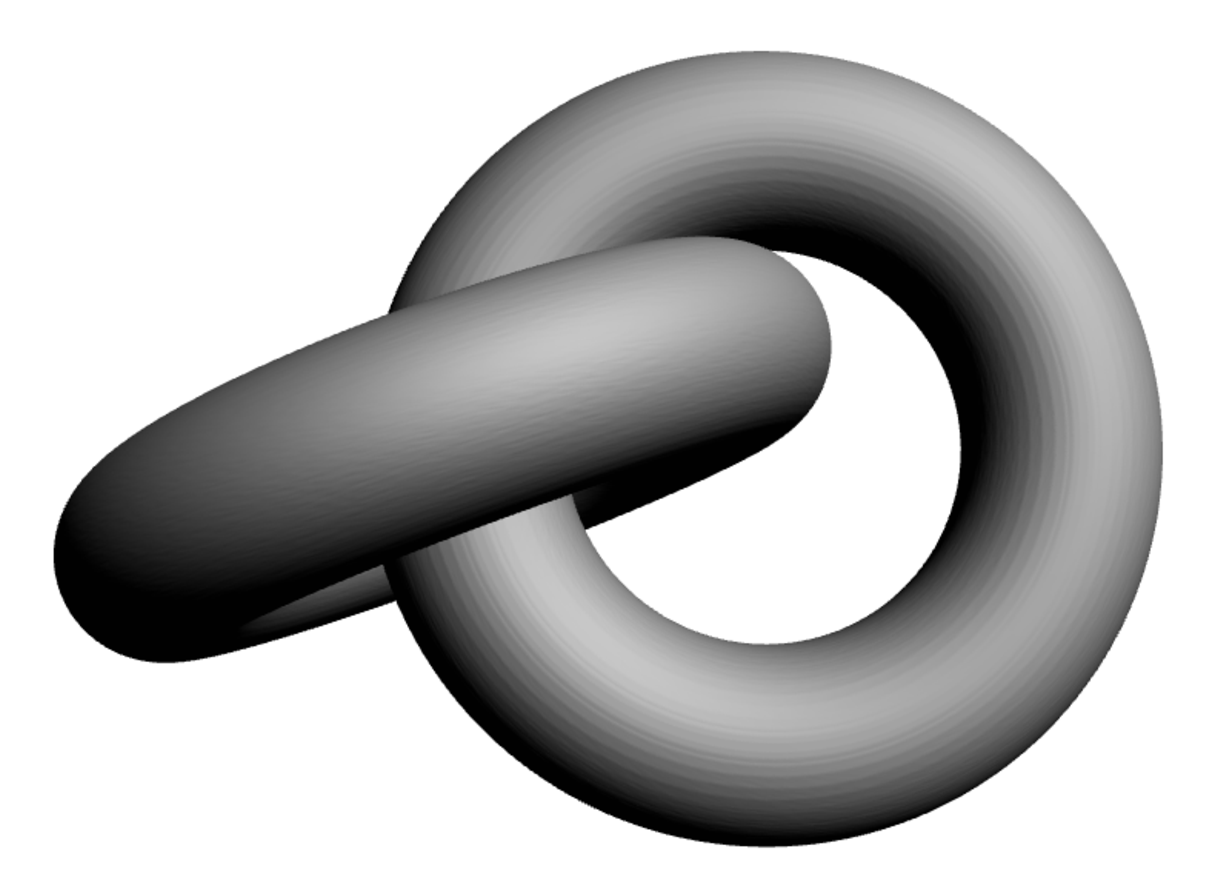
\includegraphics{modele.pdf}}{/dynamique/modele.u3d}

\mediabutton[3Dgotoview=figure_modele:0]{\fbox{Vue par défaut}}
\mediabutton[3Dgotoview=figure_modele:1]{\fbox{Vue de face}}
\mediabutton[3Dgotoview=figure_modele:2]{\fbox{Vue du maillage}}
\mediabutton[3Dgotoview=figure_modele:3]{\fbox{Vue en transparence}}

\end{center}  
\caption{Exemple de vues dynamiques
\label{figure_modele_dynamique}} 
\end{figure}


\newpage
\FloatBarrier
\LaTeX rend possible l'intégration d'images vectorielles, comme visible Figure~\ref{figure_vectorielle}. A la différence des "images matricielles" constituées de pixels, les images vectorielles sont des images numériques dans lesquelles il est possible de zoomer sans perte de qualité (sans apparition de pixel). Faites l'essai sur la Figure~\ref{figure_vectorielle} !

\begin{figure}[hbtp]
	\centering
	\def\svgwidth{1\columnwidth}
	\fontsize{10pt}{10pt}\selectfont\input{Figures/image_vectorielle.pdf_tex}
	\caption{Exemple d'image vectorielle}
	\label{figure_vectorielle}
\end{figure}



%-----------------------------------------------------------------------------------
%-----------------------------------------------------------------------------------
\FloatBarrier
\newpage

\bibliographystyle{plain}
\bibliography{bibliographie}


%%%%%%%%%%%%%%%%%%%%%%%%%%%%%%%%%%%%%%%%%%%%%%%%%%%%%%%%%%%%%%%%%%%%%%%%%%%%%%%%%%%%
%%-------------> FIN DU DOCUMENT
%%%%%%%%%%%%%%%%%%%%%%%%%%%%%%%%%%%%%%%%%%%%%%%%%%%%%%%%%%%%%%%%%%%%%%%%%%%%%%%%%%%%

\end{document}